%!TEX root =  main.tex
\setcounter{chapter}{7}
\setcounter{section}{8}
\setcounter{theorem}{0}
\setcounter{equation}{0}

\lectureheader{162}{Calculus II}{Relative orders}{\textit{Thomas' Calculus} \thesection}

\begin{remark}\,
\begin{itemize}
\item It is often necessary to compare the relative size of two functions for ``large" $x$.
\item In practice, we are usually comparing a complicated/exotic function to a simpler/more familiar one.
\item This sort of thing comes up all the time when analyzing the efficiency of algorithms and the long-term behavior of other mathematical models.
\end{itemize}
\end{remark}

\begin{definition}
Let $f$ and $g$ be functions that are defined for all $x$ sufficiently large.
We say that $f$ is \textbf{at most the order of} $g$ as $x\to \infty$, and we write
\begin{equation*}
f(x) = O(g(x)) \text{ as } x\to \infty
\end{equation*}
or we write
\begin{equation*}
f(x)\ll g(x) \text{ as } x\to \infty,
\end{equation*}
if there are constants $C, M>0$ so that $|f(x)|\le C g(x)$ for all $x\ge M$.
\end{definition}
\begin{remark}\,
\begin{itemize}
\item The constant $C$ in the definition is called the \textbf{implicit constant} since it does not appear explicitly in either notation.
\item The first notation was invented by Bachmann and Landau while the second notation was invented by Vinogradov.
\item \textit{Thomas' Calculus} (your textbook) does not recognize the second notation.
\item Your professor prefers the Vinogradov notation for at least the following reasons.
\begin{enumerate}
\item If written sloppily, big-Oh is easily confused with little-Oh.  See below.
\item The $\ll$ symbol reminds us that what really underlies the notation is an inequality.
\item We are used to statements with equals signs being symmetric, but this is not necessarily so with the equals sign in the big-Oh notation.
\item Occasionally, students will confuse $O$ with a function and think we are talking about composition of functions.
\end{enumerate}
\item Caution: To say that $f(x) = O(g(x))$ as $x\to \infty$ does not necessarily imply that $g(x)$ is ever larger than $f(x)$.
\end{itemize}
\end{remark}

\newpage

\begin{example}\label{big-oh example}
Show that $x+\sin x = O(x)$ as $x\to\infty$.
\end{example}
\ifdefined\SOLUTION
\SOLUTION{
For all $x \geq 1$,
\begin{equation*}
    x + \sin{x} \leq x + 1 \leq x + x = 2x.
\end{equation*}
So, taking $M = 1$ and $C = 2$, we get $x + \sin{x} = O(x)$ as $x\to \infty$.
Alternatively, we could say that $x+\sin x \ll x$ as $x\to\infty$.
%Note that it is also true to say that
%\begin{equation*}
%    x + \sin{x} \leq x + 1 \leq x + \frac{1}{4}x = \frac{5}{4}x
%\end{equation*}
%for all $x \geq 4$.
%So, $M = 4$ and $C = 5/4$ also would have worked.
%You don't have to find the ``best" constants, but you do need to make a convincing argument that your constants work.
}
\fi
\vfill

\begin{example}
Show that $\E^{-x^2/2}\ll \E^{-x}$ as $x\to\infty$.
\end{example}
\ifdefined\SOLUTION
\SOLUTION{
Note that $x\le x^2/2$ if and only if $0\le x^2/2-x = \frac{1}{2}x(x-2)$.
Whence, for all $x\ge 2$, it follows that
\begin{equation*}
0<x\le x^2/2,
\end{equation*}
and hence
\begin{equation*}
1<\E^x\le \E^{x^2/2}.
\end{equation*}
Therefore, taking $M=2$ and $C=1$, we see that $\E^{-x^2/2}\ll \E^{-x}$ as $x\to\infty$.
}
\fi

\vfill

\begin{example}
Show that $x^2\ll (\ln x)^{\ln x}$ as $x\to\infty$.
\end{example}
\ifdefined\SOLUTION
\SOLUTION{
When comparing these functions, it is helpful to note that 
\begin{align*}
x^2 &= \exp(2\ln x),\\
(\ln x)^{\ln x} &= \exp((\ln x)\ln\ln x).
\end{align*}
Since the natural exponential is increasing, we just need to show that $\ln\ln x\ge 2$ for all $x$ larger than some cutoff.
Using the fact that the natural logarithm is increasing on its domain, we easily have $\ln\ln x\ge 2$ for all $x\ge M=\E^{\E^2}\approx 1618$.
Therefore, $x^2\ll (\ln x)^{\ln x}$ as $x\to\infty$.
}
\fi

\vfill

\newpage

\begin{definition}
Let $f$ and $g$ be functions that are positive for all $x$ sufficiently large.
We say that $f$ is \textbf{of the same order as} $g$ as $x\to \infty$, and we write
\begin{equation*}
f(x) = \Theta(g(x)) \text{ as } x\to\infty
\end{equation*}
or we write
\begin{equation*}
f(x) \asymp g(x) \text{ as } x\to \infty,
\end{equation*}
if $f(x)\ll g(x)$ and $g(x)\ll f(x)$ as $x\to \infty$.
\end{definition}

\begin{remark}
\textit{Thomas' Calculus} (your textbook) does not recognize either of these notations, but the concept is still there.
\end{remark}

\begin{theorem}
If $L$ is a nonzero real number and $\DS\lim_{x\to\infty}\frac{f(x)}{g(x)} = L$, then $f(x)\asymp g(x)$ as $x\to\infty$.
\end{theorem}


\begin{example}
Show that $(\sqrt{2x+4}+\cos x)^3\asymp x^{3/2}$ as $x\to\infty$.
\end{example}
\ifdefined\SOLUTION
\SOLUTION[Solution]{
Since
\begin{equation*}
\begin{split}
\lim_{x\to\infty}\frac{(\sqrt{2x+4}+\cos x)^3}{x^{3/2}}
&=\lim_{x\to\infty}\left(\frac{\sqrt{2x+4}}{\sqrt x} + \frac{\cos x}{\sqrt x}\right)^3\\
&=\lim_{x\to\infty}\left(\sqrt{2+\frac{4}{x}} + \frac{\cos x}{\sqrt x}\right)^3\\
& = \left(\sqrt{2+0}+0\right)^3 = \sqrt 2\ne 0,
\end{split}
\end{equation*}
it follows that $(\sqrt{2x+4}+\cos x)^3\asymp x^{3/2}$ as $x\to\infty$.
}
\else
\fi
\vfill

\newpage

\begin{remark}\,
\begin{itemize}
\item In the previous example, we used a limit to show that $(\sqrt{2x+4}+\cos x)^3\asymp x^{3/2}$ as $x\to\infty$.
\item In other words, we showed that
\begin{equation*}
x^{3/2} \ll (\sqrt{2x+4}+\cos x)^3\ll x^{3/2} \text{ as } x\to\infty.
\end{equation*}
\item In other words, $f(x) = (\sqrt{2x+4}+\cos x)^3$ is trapped between to multiples of $g(x)=x^{3/2}$ for all sufficiently large $x$.
\item By using the limit, we were able to bypass the need to work out
\begin{enumerate}
\item which constant multiples we wanted to use, and
\item how large $x$ needs to be so that the inequalities ``kick in."
\end{enumerate}
\item The graph below indicates a choice of constants that we could probably use if we were willing to engage in finer analysis of inequalities as in the first several examples.
\end{itemize}
\end{remark}

\begin{figure}[H]
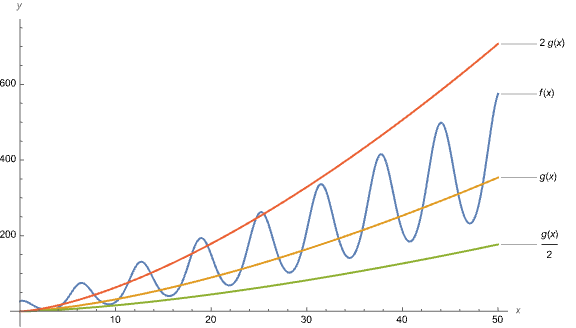
\includegraphics[width=6.5in]{img/example2}\caption{$f(x) = (\sqrt{2x+4}+\cos x)^3$ and $g(x) = x^{3/2}$}
\end{figure}

\newpage

\begin{example}
Compare the growth rates of $\E^x$ and $\cosh x$ as $x\to\infty$.
\end{example}
\ifdefined\SOLUTION
\SOLUTION[Solution]{
Let's ``race them to $\infty$."
Observe that
\begin{equation*}
\begin{split}
    \lim_{x\to \infty} \frac{\cosh{x}}{\E^x}
    = \lim_{x\to \infty} \frac{\left(\frac{\E^x+\E^{-x}}{2}\right)}{\E^x}
    = \frac{1}{2} \lim_{x\to \infty} (1 + \E^{-2x}) = \frac{1}{2}\ne 0.
\end{split}
\end{equation*}
So, $\E^x \asymp \cosh{x}$ as $x\to \infty.$
}
\else
\fi
\vfill

\begin{definition}
Let $f$ and $g$ be functions that are defined for all $x$ sufficiently large.
We say that $f$ is \textbf{of smaller order than} $g$ as $x\to \infty$, and we write
\begin{equation*}
f(x) = o(g(x)) \text{ as } x\to \infty
\end{equation*}
or we write
\begin{equation*}
f(x) \lll g(x) \text{ as } x\to\infty,
\end{equation*}
if
\begin{equation*}
\lim_{x\to\infty}\frac{f(x)}{g(x)} = 0.
\end{equation*}
\end{definition}

\begin{remark}\,
\begin{itemize}
\item If $f(x)\lll g(x)$ as $x\to\infty$, then the definition of limit implies that for every $\epsilon>0$, there is an $M>0$ so that
\begin{equation*}
x\ge M\implies |f(x)|\le \epsilon |g(x)|,
\end{equation*}
i.e., $|f(x)|$ is \underline{eventually} smaller than every positive multiple of $|g(x)|$.
%\item The first notation was invented by Bachmann and Landau, and it is read ``$f(x)$ is little-Oh of $g(x)$ as $x$ tends to infinity."
%\item The second notation was invented by Vinogradov, and it is read ``$f(x)$ is less-than-less-than-less-than $g(x)$ as $x$ tends to infinity."
\item \textit{Thomas' Calculus} (your textbook) does not recognize the second notation.
\item If $\DS\lim_{x\to\infty}\frac{f(x)}{g(x)} = \infty$, then it follows that $f(x)\ggg g(x)$ as $x\to\infty$.
\end{itemize}
\end{remark}

\begin{example}
Show that $x^2\lll \E^x$ as $x\to\infty$.
\end{example}

\ifdefined\SOLUTION
\SOLUTION[Solution]{
Using L'H\^opital's rule, we find that
\begin{equation*}
    \lim_{x\to \infty} \frac{x^2}{\E^x}
    = \lim_{x\to \infty} \frac{2x}{\E^x}
    = \lim_{x\to \infty} \frac{2}{\E^x}
    = 0.
\end{equation*}
Therefore, we may say that $x^2 \lll \E^x$ as $x\to \infty$, or we can say $x^2 = o(\E^x)$ as $x\to \infty$. 
}
\fi
\vfill

\newpage

\begin{theorem}
For every (fixed) $\epsilon>0$, 
\begin{equation*}
\ln x\lll x^\epsilon
\end{equation*}
as $x\to\infty$.
\end{theorem}
\ifdefined\SOLUTION
\SOLUTION[Proof]{
Let $\epsilon > 0$. 
Then L'H\^opital's rule gives
\begin{equation*}
    \lim_{x\to \infty} \frac{\ln{x}}{x^{\epsilon}}
    = \lim_{x\to \infty} \frac{1/x}{\epsilon x^{\epsilon - 1}}
    = \lim_{x\to \infty} \frac{1}{\epsilon}\cdot \frac{1}{x^{\epsilon}} 
    = 0.
\end{equation*}
In other words, $\ln x \lll x^{\epsilon}$ as $x\to \infty$ for any $\epsilon>0$.
}
\else
\begin{proof}\,

\vspace{1.25in}
\end{proof}
\fi

\vfill

\begin{remark}\,
\begin{itemize}
\item The previous theorem tells us that although $\ln x\to\infty$ as $x\to\infty$, ultimately it does so at a much slower rate than \underline{every} power function.
\item Although, $\ln x$ is ``winning the race" for a long time, $x^{1/4}$ will \textit{eventually} leave $\ln x$ in its dust.
\end{itemize}
\end{remark}

\begin{figure}[H]
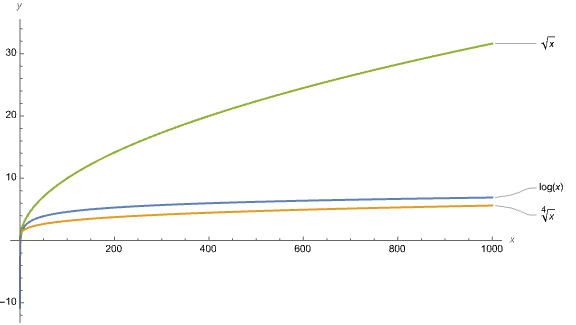
\includegraphics[width=4in]{img/log-growth}
%\begin{tikzpicture}
%\pgfplotsset{height=0.35\textheight}
%\begin{axis}[axis lines=middle, xlabel = $x$, ylabel=$y$]
%\addplot[domain=0:1000, red, line width=2pt, samples=100]{sqrt(x)};
%\addlegendentry{$y=x^{1/2}$}
%\addplot[domain=0:1000,  green, line width=2pt, samples=100]{x^(1/4)};
%\addlegendentry{$y= x^{1/4}$}
%\addplot[domain=0:1000,  blue, line width=2pt, samples=100]{ln(x)};
%\addlegendentry{$y=\ln x$}
%\end{axis}
%\end{tikzpicture}
\end{figure}

\begin{figure}[H]
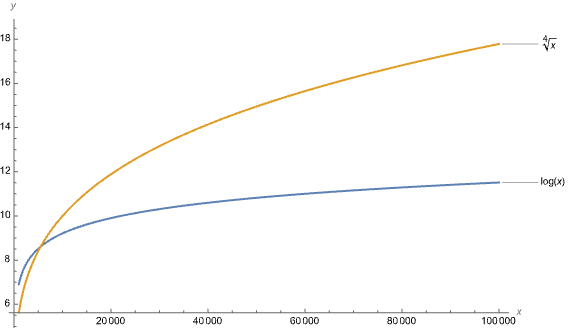
\includegraphics[width=4in]{img/log-growth2}
%\begin{tikzpicture}
%\pgfplotsset{height=0.35\textheight}
%\begin{axis}[axis lines=left, xlabel = $x$, ylabel=$y$]
%\addplot[domain=0:100000,  green, line width=2pt, samples=100]{x^(1/4)};
%\addlegendentry{$y= x^{1/4}$}
%\addplot[domain=0:100000,  blue, line width=2pt, samples=100]{ln(x)};
%\addlegendentry{$y=\ln x$}
%\end{axis}
%\end{tikzpicture}
\end{figure}


\newpage

\begin{corollary}
For every (fixed) $M>0$,
\begin{equation*}
x^M\lll\exp(x)
\end{equation*}
as $x\to\infty$.
\end{corollary}

\ifdefined\SOLUTION
\SOLUTION[Proof]{
Let $M>0$.
By the previous theorem and the change of variables $y=\exp x$, we have
\begin{equation*}
\lim_{x\to\infty}\frac{x^M}{\exp x}
=\lim_{y\to\infty}\frac{(\ln y)^M}{y}
=\lim_{y\to\infty}\left(\frac{\ln y}{y^{1/M}}\right)^M
=0^M
=0.
\end{equation*}
}
\else
\begin{proof}\,

\vspace{1.5in}
\end{proof}
\fi

\begin{definition}
Let $f$ and $g$ be functions that are defined for all $x$ sufficiently large.
We say that $f$ is \textbf{asymptotic to} $g$ as $x\to \infty$, and we write
\begin{equation*}
f(x) \sim g(x) \text{ as } x\to \infty
\end{equation*}
if
\begin{equation*}
\lim_{x\to\infty}\frac{f(x)}{g(x)} = 1.
\end{equation*}
\end{definition}

\begin{remark}\,
\begin{itemize}
\item The above definition says that $f$ and $g$ have an even closer relationship than merely having the same order.
\item To say that $f(x)\sim g(x)$ as $x\to \infty$  is to say that $g(x)$ is a ``good approximation" to $f(x)$ in the sense that the \underline{relative error} can be made arbitrarily small by choosing a large enough $x$, i.e., 
\begin{equation*}
\left|\frac{f(x) - g(x)}{f(x)}\right|\to 0
\end{equation*}
as $x\to\infty$.
\item \textit{Thomas' Calculus} (your textbook) does not mention this concept at all, but it is extremely useful.
\end{itemize}
\end{remark}

\begin{example}
Show that $\sinh x\sim \frac{1}{2}\E^x$ as $x\to\infty$.
\end{example}
\ifdefined\SOLUTION
\SOLUTION[Solution]{
Let's race:
\begin{equation*}
\lim_{x\to\infty}\frac{\sinh x}{\E^x/2} 
=\lim_{x\to\infty}\frac{\frac{\E^x-\E^{-x}}{2}}{\E^x/2} 
=\lim_{x\to\infty}\left(1- \E^{-2x}\right) = 1.
\end{equation*}
In other words, $\sinh x\sim \frac{1}{2}\E^x$ as $x\to\infty$.
}
\fi
